%!TEX root = ../thesis.tex
\section{構造解析}
設計したアームには,7つの板金部品を使用している.それぞれの部品は,軽量化と強度を考慮し設計している.特に,肩部の部品1と部品2(図\ref{fig:shoulder})は,最も負荷がかかる部位であるため,inventor上で構造解析を行い,強度を確認している.以下に,各部品の構造解析について述べる.
\begin{figure}[h]
  \centering
  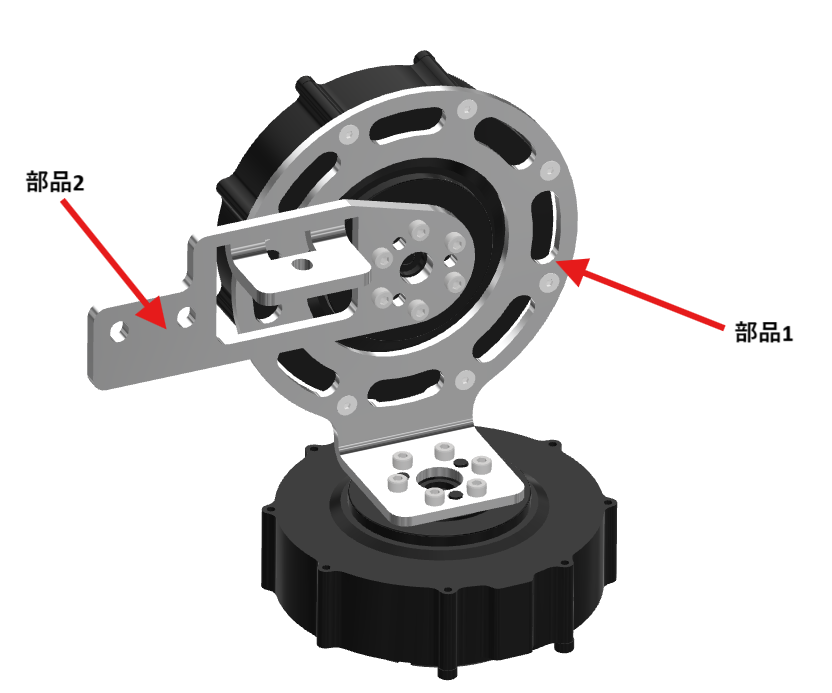
\includegraphics[width=10cm]{images/design/shoulder.png}
  \caption{肩部の構成}
  \label{fig:shoulder}
\end{figure}

※※ ここに構造解析の結果を乗せる.構造解析がしっかりできていなかったので,やり直し中.

\newpage